\documentclass[a4paper,12pt]{article}
\usepackage[T2A]{fontenc}
\usepackage[utf8]{inputenc}
\usepackage[english,russian]{babel}
\usepackage{circuitikz}
\usepackage{wrapfig}
\usepackage{makecell}
\parindent=0ex
\usepackage{tabularx}
\usepackage{graphicx}
\usepackage{gensymb}
\usepackage{cancel}
\usepackage{amsmath,amsfonts,amssymb,amsthm,mathtools}
\usepackage{tikz}
\usetikzlibrary{intersections}
\usetikzlibrary{arrows.meta}
\usetikzlibrary{calc,angles,positioning}
\usepackage{float}
\graphicspath{ {C:/Users/George/Documents/MIPT_TEX/LAB_1_4_1} }



\begin{document}
	\begin{center}
		МОСКОВСКИЙ ФИЗИКО-ТЕХНИЧЕСКИЙ ИНСТИТУТ (НАЦИОНАЛЬНЫЙ ИССЛЕДОВАТЕЛЬСКИЙ УНИВЕРСИТЕТ) \\
		
		
		\hfill \break
		Факультет обшей и прикладной физики\\
		\vspace{2.5cm}
		\large{\textbf{Отчёт по лабораторной работе 1.2.3 <<Определение моментов инерции твёрдых тел с помощью трифилярного подвеса>>}}\\
		\hfill \break
		\\
	\end{center}
	
	\vspace{5cm}
	
	\begin{flushright}
		Выполнил:\\
		Студент гр. Б02-304\\
		Головинов. Г.А.
	\end{flushright}
	
	\vfill
	
	
	\begin{center} Долгопрудный, 2023 \end{center}
	
	\thispagestyle{empty}
	\newpage
	\pagenumbering{arabic}
	
	\section{Аннотация}
	\paragraph{Цель работы:} \hspace{-4mm} Измерение момента инерции некоторых твёрдых тел, сравнение полученных данных с теоретическими, а также проверка справедливости теоремы Гюйгенса-Штейнера.
	\paragraph{Используемые инструменты:} \hspace{-4mm} Трифилярный подвес, секундомер, счётчик числа колебаний, набор твёрдых тел.\\
	\section{Основные теоретические сведения}
	Установка, используемая в работе называется трифилярным подвесом и представляет собой массивный диск, подвешенный на трех нитях к другому, меньшему диску, на большой высоте. Такая установка может совершать вращательные колебания небольшой амплитуды.
	\begin{figure}[H]
		\centering
		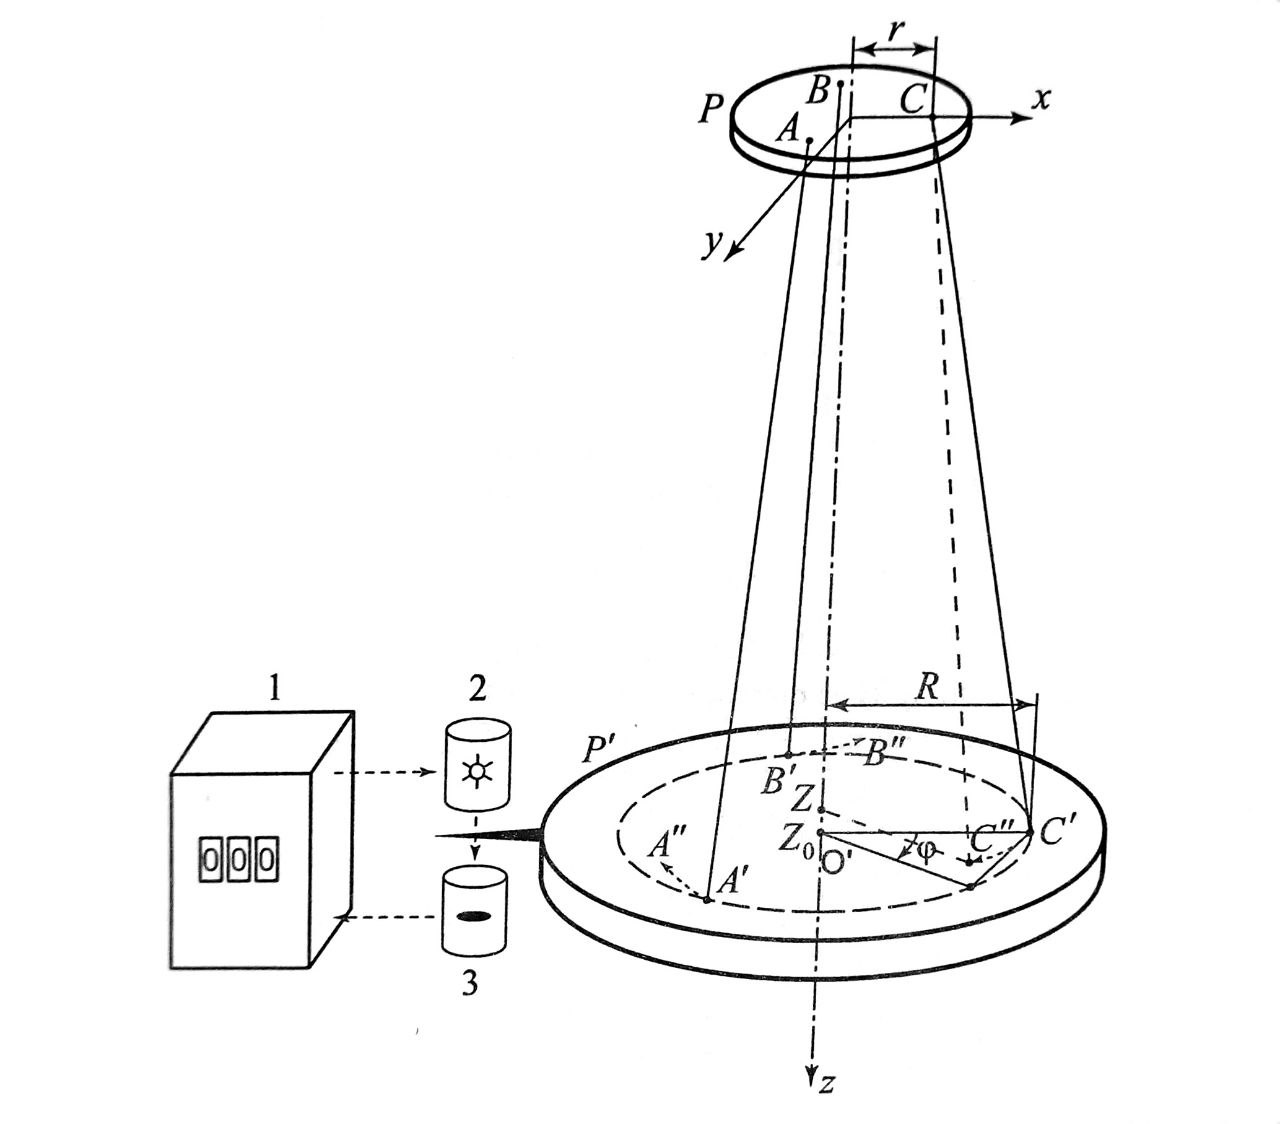
\includegraphics[width=0.7\linewidth]{fig1}
		\caption[]{Трифилярный подвес}
		\label{fig:fig1}
	\end{figure}
	
	На рисунке 1,2,3 - установка с секундомером и счётчиком числа колебаний.\\
	
	\paragraph{Момент инерции}
	Мерой инертности тела при вращательном движении вокруг некоторой оси является момент инерции, который по определению равен:
	\begin{equation}
		I=\int r^2dm
	\end{equation}
	Где $r$ - расстояние части тела массой $dm$ до оси вращения\\
	
	То есть для некоторых тел известной массы и точных размеров мы можем посчитать момент инерции относительно некоторой оси. Например диск и ось, проходящая перпендикулярно ему через его центр. Однако если требуется определить момент инерции тела более сложного (в геометрическом смысле слова), то тут потребуется использовать теорему Гюйгенса-Штейнера.
	
	\paragraph{Теорема Гюйгенса-Штейнера}
	Эта теорема гласит, что для любого твёрдого тела справедливо соотношение:
	\begin{equation}
		I_A=I_C+mh^2
	\end{equation}
	где $I_A$ - момент инерции относительно некоторой произвольной оси параллельной оси, проходящей через центр масс этого тела, $I_C$ - момент инерции этого тела относительно оси, проходящей через центр масс, $h$ - расстояние между этими осями, $m$ - масса тела.\\
	
	С помощью этого соотношения можно найти моменты инерции более сложных комбинаций тело-ось. Например: сегмент диска и ось, проходящая через его центр масс или шар и ось, проходящая к нему по касательной.\\
	
	Теорема достаточно легко доказывается математически, однако в этой работе мы проверим ее справедливость экспериментально.
	
	\paragraph{Аддитивность моментов инерции}
	
	Следствием из определения момента инерции очевидно является его аддитивность. То есть если мы возьмем систему из нескольких тел и рассмотрим ее вращение относительно некоторой оси, то момент инерции системы относительно этой оси будет равен алгебраической сумме моментов инерции каждого тела относительно этой оси по отдельности.
	\newpage
	\paragraph{Соотношения необходимые в работе}
	\begin{equation}
		I=kmT^2
	\end{equation}
	где $m$ - масса, $T$ - период, $k$ - коэффициент, определяемый:
	\begin{equation}
		k=\frac{gRr}{4\pi^2z_0}
	\end{equation}
	
	\section{Результаты измерений и обработка данных}
	Перед непосредственным выполнением работы требуется определить насколько сильно затухают колебания нашей установки, найти наиболее оптимальную амплитуду колебаний, а также определить момент инерции самой платформы.
	
	\begin{table}[H]
		\centering
		\caption{Полученные значения периода колебаний для каждой амплитуды}
		\begin{tabular}{|c|c|c|c|}
			\hline
			$A \degree$ & $N$ & $t$, c & $T$, c \\
			\hline
			30 & 5 & 22.26 & 4.4520 \\
			\hline
			20 & 5 & 22.11 & 4.4220 \\
			\hline
			15 & 5 & 22.07 & 4.4140 \\
			\hline
			10 & 5 & 22.04 & 4.4080 \\
			\hline
			5 & 5 & 22.00 & 4.4000 \\
			\hline
		\end{tabular}
	\end{table}
	
	Полученные периоды почти не различаются, однако заметно, что наилучшие показания наблюдаются при амплитуде около 10-15 градусов, так как при низких амплитудах сильнее влияет затухание, а при высоких амплитудах заметны эффекты раскачивания платформы. Рабочим диапазоном определим 5-15 градусов.\\
	
	На этом этапе можно было просто посчитать один раз случайную погрешность измерений и потом ее использовать для каждого последующего, однако было решено каждый раз делать по 5 измерений и определять погрешность каждый раз заново. Учитывая точность секундомера это не является обязательным пунктом.\\
	
	\paragraph{Важная оговорка}
	
	Далее момент инерции -- значит момент инерции тела относительно оси симметрии (так как мы располагали тела в центре платформы)
	
	\paragraph{Погрешности}
	Погрешность коэффициента $k$ рассчитаем по следующей формуле:
	\begin{equation}
		\sigma_k=k\sqrt{\left(\frac{\sigma_r}{r}\right)^2+\left(\frac{\sigma_R}{R}\right)^2+\left(\frac{\sigma_{z_0}}{z_0}\right)^2}=0.00000716
	\end{equation}
	Единицы в СИ.\\
	
	Погрешность периода для каждого измерения будем считать как
	\begin{equation}
		\sigma_T^2=\frac{1}{4}\sum (T-\bar{T})^2
	\end{equation}
	
	Погрешность момента инерции будем считать
	\begin{equation}
		\sigma_I=I\sqrt{\left(\frac{\sigma_k}{k}\right)^2+\left(\frac{\sigma_m}{m}\right)^2+\left(2\frac{\sigma_T}{T}\right)^2}
	\end{equation}
	
	\paragraph{Момент инерции пустой платформы}
	Платформа представляет собой диск. Его масса была нам известна заранее и составила $m=1026,4\pm 0,5$ г. Для диска момент инерции $I=\frac{1}{2}mR^2$\\
	
	Таким образом теоретический момент инерции составил $0.008095$ кг$\cdot$м$^2$, а экспериментальный $(0.008019\pm 0.000161)$ кг$\cdot$м$^2$ ($\varepsilon=2\%$), расхождение с теоретическим значением менее $1\%$, попадает в интервал $\pm 1\sigma$.\\
	
	\paragraph{Кольцо (полый цилиндр)}
	Первым исследуемым телом стало кольцо (тонкостенный цилиндр), его момент инерции $I=\frac{1}{2}m(R^2+r^2)$\\
	
	Для кольца теоретическое значение момента инерции равно $0.004282$ кг$\cdot$м$^2$. Экспериментально (вычитая платформу) получим $(0.004398\pm0.000223)$ кг$\cdot$м$^2$ ($\varepsilon=1.7\%$), расхождение с теоретическим значением $2.6\%$, что не попадает в интервал $\pm 1 \sigma$\\
	
	\paragraph{Диск}\mbox{}\\
	
	Вторым исследуемым телом стал диск, его момент инерции $I=\frac{1}{2}mR^2$\\
	
	Для диска теоретическое значение момента инерции $0.002111$ кг$\cdot$м$^2$. Экспериментально (вычитая платформу) получим $(0.002071\pm 0.000182)$ кг$\cdot$м$^2$ ($\varepsilon=1.7\%$), расхождение с теоретическим $1.9\%$, что чуть-чуть не попадает в интервал $\pm 1 \sigma$	
	
	\paragraph{Кольцо и Диск}
	Вместе эти два тела должны иметь момент инерции $0.006393$ кг$\cdot$м$^2$. Экспериментально получим $(0.006482\pm 0.000268)$ кг$\cdot$м$^2$ ($\varepsilon=1.8\%$), расхождение с теоретическим значением менее $1.4\%$, что попадает в интервал $\pm 1 \sigma$
	
	\paragraph{Аддитивность моментов инерции}
	
	В инструкции к работе неясно сказано как выполнять этот пункт, поэтому был выбран следующий способ:\\
	
	Не вычитая платформы (мы как бы не знаем про аддитивность) в каждом из измерений диска и кольца по отдельности мы их сложим, если аддитивность выполняется, то мы получим $I$ кольца, диска и $2I$ платформы. Если мы из этого вычтем значение, полученное для кольца и диска вместе, то должны получить $I$ платформы.\\
	
	Таким способом мы получим $0.008081\pm 0.000124$ кг$\cdot$м$^2$ (погрешность по $\chi^2$) $\varepsilon=1.5\%$. Расхождение с теоретическим значением $I$ пустой платформы $0.167\%$.
	
	\paragraph{Теорема Гюйгенса Штейнера}
	Нам были предоставлены две половины диска (точнее сказать цилиндра), которые мы можем раздвигать на расстояние $h$ от центра платформы (не смещая при этом центр масс системы). Тогда согласно теореме Гюйгенса-Штейнера момент инерции системы будет равен $I=I_{platform}+I_{disk}+mh^2$, где $m$ - масса диска, $I_disk$ - момент инерции диска относительно оси, проходящей перпендикулярно ему через его центр масс.\\
	
	Погрешность периода возьмем по $\chi^2$ из предыдущих пунктов (про моменты инерции других тел)\\
	
	Если мы построим зависимость $I(h^2)$, то должны получить прямую $y=ax+b$, где $a$ - масса диска, а $b$ - момент инерции платформы и диска.\\
	
	Аппроксимируя по методу $\chi^2$ получим $a=(1.53895\pm 0.02455)$ кг, $b=(0.009701\pm 0.000045)$ кг$\cdot$м$^2$\\
	
	Масса диска определена с погрешностью $\varepsilon=1.5\%$, расхождение с известным значением меньше $0.85\%$, что попадает в интервал $\pm 1\sigma$.\\
	
	Тогда момент инерции диска $I=(0.001606\pm 0.000045)$ кг$\cdot$м$^2$, а экспериментально (при $h=0$) $I=(0.001544\pm 0.000172)$ кг$\cdot$м$^2$, относительная разница $3.8\%$. Итоговый момент инерции диска $I=(0.001575\pm 0.000044)$ кг$\cdot$м$^2$.
	
	\begin{figure}[H]
		\centering
		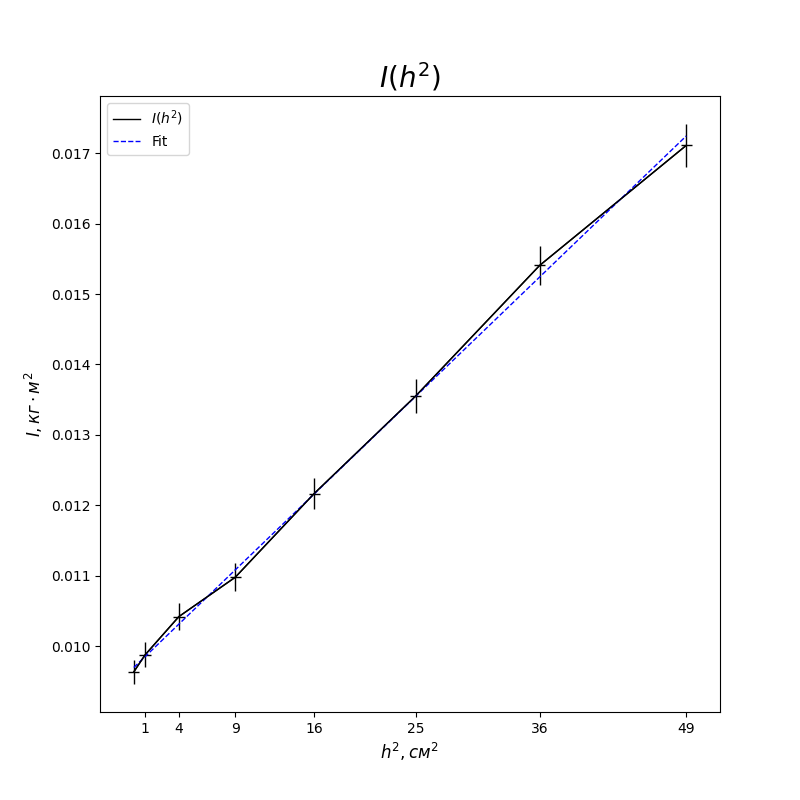
\includegraphics[width=\linewidth]{Figure_1}
		\caption{Зависимость момента инерции от квадрата смещения от центра платформы}
		\label{fig:figure1}
	\end{figure}
	
	
	\section{Обсуждение результатов и выводы}
	
	В ходе работы мы измерили экспериментально и теоретически моменты инерции различных твёрдых тел с помощью трифилярного подвеса. Практически для всех тел теоретические значения попали в интервал $\pm 1\sigma$ от экспериментальных, что говорит об достаточно хорошей оценке систематической погрешности, однако по традиции, в некоторых случаях, она была недооценена.\\
	
	Кроме того, в ходе работы мы проверили справедливость аддитивности моментов инерции нескольких твёрдых тел.\\
	
	Мы проверили справедливость теоремы Гюйгенса-Штейнера с помощью построения графика $I(h^2)$ для двух половинок диска, смещенного на некоторое расстояние $h$ от центра платформы. Масса диска и его момент инерции были определены с достаточно большой точностью (масса менее $0.85\%$, момент инерции менее $3.8\%$)
\end{document}